\chapter{準備}\label{chapter:2}
\section{ペンシルパズルに関する諸概念の定義}
\subsection{用語の定義}
この節ではペンシルパズルにおける用語を定義する.

ただし,ペンシルパズルとは「サイズ$m\times n$の平面グリッドが盤面として与えられ,パズルルールに定められた条件と,その解答ステップにおいて明らかになっている解から格子点,細胞,辺のいずれかの未知情報に論理的推測から解を書き込み,全ての格子点,細胞,辺がパズルルールに定められた条件を満たす完成盤面へと解く行為と,その問題やルールなどを一括りに呼ぶ概念」とし,明確な定義は行わずあくまで概念として以下もペンシルパズルという用語を使用する.

ここで,ペンシルパズルにおいて具体的なパズルルールを与えた際に,そのパズルルールに則った問題を考えることができる.その問題にかかわる概念として完成盤面と未完成盤面の定義を行う.

\begin{definition}\label{definition:FinishedBoard}\textup{\textgt{完成盤面}}

  全ての格子点,細胞,辺がパズルルールに定められた条件を満たしている盤面
\end{definition}

\vskip\baselineskip
\begin{definition}\label{definition:UnfinishedBoard}\textup{\textgt{未完成盤面}}

  各未知情報がその未完成盤面に対応する完成盤面の解と一対一に対応するような盤面.(\textgt{唯一解})
\end{definition}
\vskip\baselineskip

上の記述より,一つの完成盤面には複数の未完成盤面が対応する.(一つの操作(未知情報に解を書き込む)を課した未完成盤面もまた未完成盤面.)

つまり,未完成盤面から完成盤面への写像が(そのパズルルールに対し)ただ一つ存在すれば,その未完成盤面の集合全体は与えたパズルルールの「問題である」と言える.

\subsection{盤面上の情報に関する概念の数学的定義}
この節ではペンシルパズルにおける盤面上の情報に関する各概念を数学的に定義する.ここで定義するものは全て直感的な定義と違わないように行う.


平面グリッドを与えたとき,ペンシルパズルの盤面には左上から各格子点に対し座標$(i,j)$を割り振ることができる.そうした時,グリッドにおける格子点,細胞,辺に対して下図(図\ref{fig:VariableAtBoard})で表されるように変数を与えることができるが,これを数学的に定義する.各格子点,辺,細胞を構成する各座標の集合と$(i,j)$の間にはそれぞれ以下のものが定義できる.
\begin{definition}\label{definition:VariableAtBoard}\textup{\textgt{盤面上の変数}}
  \begin{align}
    p(i,j)\coloneqq & \{(i,j)\}                              & \\
    c(i,j)\coloneqq & \{(i,j), (i,j+1), (i+1,j), (i+1,j+1)\} & \\
    h(i,j)\coloneqq & \{(i,j), (i,j+1)\}                     & \\
    v(i,j)\coloneqq & \{(i,j), (i+1,j)\}                     &
  \end{align}

  ただし,$h(i,j),v(i,j)$の詳細に興味がない場合は,それらを合わせて$e(i,j)$と記述する.また,盤面上の変数の詳細そのものに興味がない場合は上記のもの全て合わせて$\lambda(i,j)$と記述する.
\end{definition}
\vskip\baselineskip
このような包含写像が存在し,これを$p(i,j),c(i,j),h(i,j),v(i,j)$の定義とし,このような添え字付きの変数を改めて格子点,細胞,辺と呼び,これらをまとめた概念として盤面上の変数と呼ぶこととする.

\begin{figure}[htbp]
  \centering
  \includegraphics[width=5cm,clip]{fig/define.png}
  \caption{まだ作成できておらず,内容が少し異なりますがイメージのためにつけておきます.}
  \label{fig:VariableAtBoard}
\end{figure}

ペンシルパズルにおいて,盤面上の変数に対して,ソルバーは未知情報に対して解を書き込むことが前提にあるので,パズルルールを定義するためには,解がどのような集合の元に含まれるかを定義する必要がある.そのために以下で$\mathbf{codomain}$という用語を用いて解集合を定義する.

\begin{definition}\label{definition:Codomain}\textup{$\mathbf{codomain}$}

  盤面上の変数の集合に対し一対一に対応する解の列の要素がとりうる値の集合のことを$\mathbf{codomain}$と呼ぶこととする.格子点,細胞,辺の$\mathbf{codomain}$を表す集合として$\mathbb{P},\mathbb{C},\mathbb{H},\mathbb{V}$を用いる.$\mathbb{H},\mathbb{V}$の$\mathbf{codomain}$が一致している場合にはまとめて$\mathbb{E}$と記述する.$\mathbf{codomain}$の詳細に興味がない場合はそれら集合を含意するものとして$\Lambda$を使用する.
\end{definition}

\vskip\baselineskip
ここで,盤面上の変数に対してそれぞれ解として具体的な値(1や3などの数値,あるいは$x_1$などの記号)が対応するがその解は列をなしていて同一の値が含んだ列となることがある.よって$\mathbf{codomain}$と解の列は同一視できないことに注意する.
以下に既存のパズルルールのスリザーリンクを例として用いる.ただし,スリザーリンクのパズルルールは以下のものである.\cite{web:SlitherLink}

\begin{enumerate}
  \item 点と点の間にタテヨコに線を引き,全体で1つの輪っかを作りましょう.
  \item 4つの点で作られた正方形の中にある数字は,その正方形の辺に引く線の数を表しています.数字のない正方形には,何本の線を引くかわかりません.
  \item 線を交差させたり,枝分かれさせたりしてはいけません.
\end{enumerate}

\begin{figure}[htbp]
  \centering
  \includegraphics[width=5cm]{fig/slitherlink.png}
  \caption{スリザーリンクの完成盤面}
\end{figure}




\begin{example}\label{example:SlitherLinkCodomain}\textup{スリザーリンクの$\mathbf{codomain}$}

  スリザーリンクにおいては,$\mathbf{codomain}$は以下のように表すことができる.しかし辺が「書かれている」時は1,「書かれていない」時は0に対応させるものとする.
  \begin{equation}
    \mathbf{codomain}\colon
    \left\{
    \begin{aligned}
      \mathbb{P} = & \{null\}      & \\
      \mathbb{C} = & \{0,1,2,3,4\} & \\
      \mathbb{E} = & \{0,1\}       &
    \end{aligned}
    \right.
  \end{equation}
\end{example}
\vskip\baselineskip

以上のように$\mathbf{codomain}$を考えることにより,盤面上の変数の各集合から,解集合($\mathbf{codomain}$)に送る写像を考えることができる.

\begin{definition}\label{definition:Mapping}\textup{盤面上の変数に解を対応させる写像}

  \begin{equation}
    \begin{array}{rccc}
      \bm{p}\colon & \{p(i,j)\}            & \longrightarrow & \mathbb{P}            \\
                   & \rotatebox{90}{$\in$} &                 & \rotatebox{90}{$\in$} \\
                   & p(i,j)                & \longmapsto     & p_{i,j}
    \end{array}
  \end{equation}
  \vskip\baselineskip

  \begin{equation}
    \begin{array}{rccc}
      \bm{c}\colon & \{c(i,j)\}            & \longrightarrow & \mathbb{C}            \\
                   & \rotatebox{90}{$\in$} &                 & \rotatebox{90}{$\in$} \\
                   & c(i,j)                & \longmapsto     & c_{i,j}
    \end{array}
  \end{equation}

  \vskip\baselineskip
  \begin{equation}
    \begin{array}{rccc}
      \bm{h}\colon & \{h(i,j)\}            & \longrightarrow & \mathbb{H}            \\
                   & \rotatebox{90}{$\in$} &                 & \rotatebox{90}{$\in$} \\
                   & h(i,j)                & \longmapsto     & h_{i,j}
    \end{array}
  \end{equation}

  \vskip\baselineskip
  \begin{equation}
    \begin{array}{rccc}
      \bm{v}\colon & \{v(i,j)\}            & \longrightarrow & \mathbb{V}            \\
                   & \rotatebox{90}{$\in$} &                 & \rotatebox{90}{$\in$} \\
                   & v(i,j)                & \longmapsto     & v_{i,j}
    \end{array}
  \end{equation}
  \vskip\baselineskip

  ただし,$\bm{h},\bm{v}$の詳細に興味がない場合は,それらをまとめて
  \begin{equation}
    \begin{array}{rccc}
      \bm{e}\colon & \{e(i,j)\}            & \longrightarrow & \mathbb{E}            \\
                   & \rotatebox{90}{$\in$} &                 & \rotatebox{90}{$\in$} \\
                   & e(i,j)                & \longmapsto     & e_{i,j}
    \end{array}
  \end{equation}
  と記述する.

  上記の写像の詳細に興味がない場合それらの写像全てを含意するものとして$\bm{\lambda}$を用いて

  \begin{equation}
    \begin{array}{rccc}
      \bm{\lambda}\colon & \{\lambda(i,j)\}      & \longrightarrow & \Lambda               \\
                         & \rotatebox{90}{$\in$} &                 & \rotatebox{90}{$\in$} \\
                         & \lambda(i,j)          & \longmapsto     & \lambda_{i,j}
    \end{array}
  \end{equation}
  と記述する.

\end{definition}
\vskip\baselineskip

集合論の用語を借りれば,解の列$\{\lambda_{1,1}, \lambda_{1,2},...\}(以下\{\lambda_{i,j}\}とする)$と写像$\bm{\lambda}\colon \{\lambda(i,j)\} \longrightarrow \Lambda$の間には$\bm{\lambda}(\lambda(i,j))=\lambda_{ij}$という自然な一対一対応が存在し,写像$\bm{\lambda}$は$\{\lambda(i,j)\}$によって添え字付けられた族であり,この時$\{\lambda(i,j)\}$は添字集合で,$\lambda(i,j)$はこの写像の添字である.

未完成盤面において,ソルバーにこれら写像の中で,盤面上の変数と解($\mathbf{codomain}$の元)との対応が公開されていないものを未知情報と呼び,公開されているもの及びソルバーが論理的推測により導いたものを既知情報と呼ぶこととする.

盤面上の変数とその解($\mathbf{codomain}$の元)の対応は(定義\ref{definition:Mapping})のように添字によってラベル付けされ,解同士の関係は(定義\ref{definition:Codomain})直後で記述したようにで実際に取る値の如何に関わらず別物として扱う.盤面上の変数と,その解(定義\ref{definition:Mapping})との対応が全て分かっているとき,写像はそれらの取る値を全て列として記述すれば
\begin{equation*}
  \bm{\lambda}\Leftrightarrow \{\lambda_{i,j}\}
\end{equation*}
と同一視することができる.

このような座標系と種々の定義を導入することにより,(パズルルールを与えず)codomainとして$\mathbb{P},\mathbb{C},\mathbb{E}$を与えたとき任意の盤面は
\begin{equation}\label{equation:U}
  U=\Bigl\{\{\bm{p},\bm{c},\bm{e}\}\Bigr\}=\biggl\{\Bigl\{\{p_{i,j}\},\{c_{i,j}\},\{e_{i,j}\}\Bigr\}\biggr\}
\end{equation}


なる集合の一つの元と言うことが出来る.ただし,写像$\bm{c}$などは各盤面においてただ一つ存在するものだから,ある具体的な盤面は$\{\bm{p},\bm{c},\bm{e}\}$と記述されることに注意する.また,$\lambda(i,j)$が$\lambda_{i,j}$と一対一対応することより誤解の恐れがない場合は$B \ni \lambda(i,j)$,あるいは$B\ni \lambda_{i,j}$と記述する.この時は$B$は集合として$B=\{\lambda(i,j)\}$を考え,$\lambda_{i,j}$も$\bm{\lambda}$によりBの元として扱うこととする.

ここで,ある問題を与えたとき完成盤面が満たしているべきパズルルールによって定められた条件は,そのまま式(\ref{equation:U})に条件として記述することができて,これを$\mathbf{conditions}$と呼ぶこととする.
\begin{definition}\label{definition:Conditions}\textup{$\mathbf{conditions}$}

  完成盤面において解が満たしているべき必要十分条件
\end{definition}
\vskip\baselineskip

$\mathbf{conditions}$の具体例は節(\ref{subsection:GraphDefinition})で定義するグラフと(定義\ref{definition:Function})で定義する関数を用いる必要があるため,後の節(例\ref{example:SlitherLinkConditions})で取り上げることとする.

上の$\mathbf{conditions}$を用いればあるパズルルールが存在した時,完成盤面全体の集合Xは

\begin{equation}\label{equation:X}
  X=\biggl\{\Bigl\{\{p_{ij}\},\{c_{ij}\},\{e_{ij}\}\Bigr\}\mid \rm{\mathbf{conditions}}\biggr\}
\end{equation}

と記述することができる.



式(\ref{equation:X})で定義した完成盤面から問題へと派生させるために「ソルバーに隠す盤面上の変数の解」として$\mathbf{HI(Hidden\;Information)}$を定義する.ただし,「隠す」という言葉は$\mathbf{codomain}$から$\mathbf{codomain}$にnullを加えた集合$\Lambda'=\Lambda\cup null$への写像$\phi\colon \Lambda \longrightarrow \Lambda'$を解の列に作用させることを意味することとする.

\begin{definition}\label{definition:HiddenInformation}\textup{$\mathbf{HI(Hidden\;Information)}$}

  ソルバーから隠す盤面上の変数の部分集合に対応する解の部分列.ただし,その部分集合はパズルルールによってそれが一意に定まるものではなく問題に依存するものとし,パズルルールでは$\{c_{i,j}\}$と$\{e_{i,j}\}$の部分列といったように隠す列及び部分列の情報のみを指定し,詳細は指定しないものとする.
\end{definition}

\vskip\baselineskip

\begin{example}\textup{スリザーリンクの$\mathbf{HI}$}


  \begin{equation}
    \mathbf{HI}\colon
    \left\{
    \begin{aligned}
       & \{c_{i,j}\}の部分列 \\
       & \{e_{i,j}\}
    \end{aligned}
    \right.
  \end{equation}
\end{example}

\vskip\baselineskip

完成盤面においては盤面上の変数と解が一対一に対応することにより,$\mathbb{E}$が要素として数値のみを持つ場合に限り新たに下記のような関数を導入することができる.(下図\ref{fig:cross}, \ref{fig:cycle})

\begin{definition}\textup{\textgt{関数}}\label{definition:Function}
  \begin{align}
    \bm{cross}(p(i,j))\coloneqq h_{i,j-1}+v_{i-1,j}+h_{i,j}+v_{i,j} \\
    \bm{cycle}(c(i,j))\coloneqq h_{i,j}+v_{i,j}+h_{i+1,j}+v_{i,j+1}
  \end{align}
\end{definition}
\begin{figure}[htbp]\label{fig:cross}
  \centering
  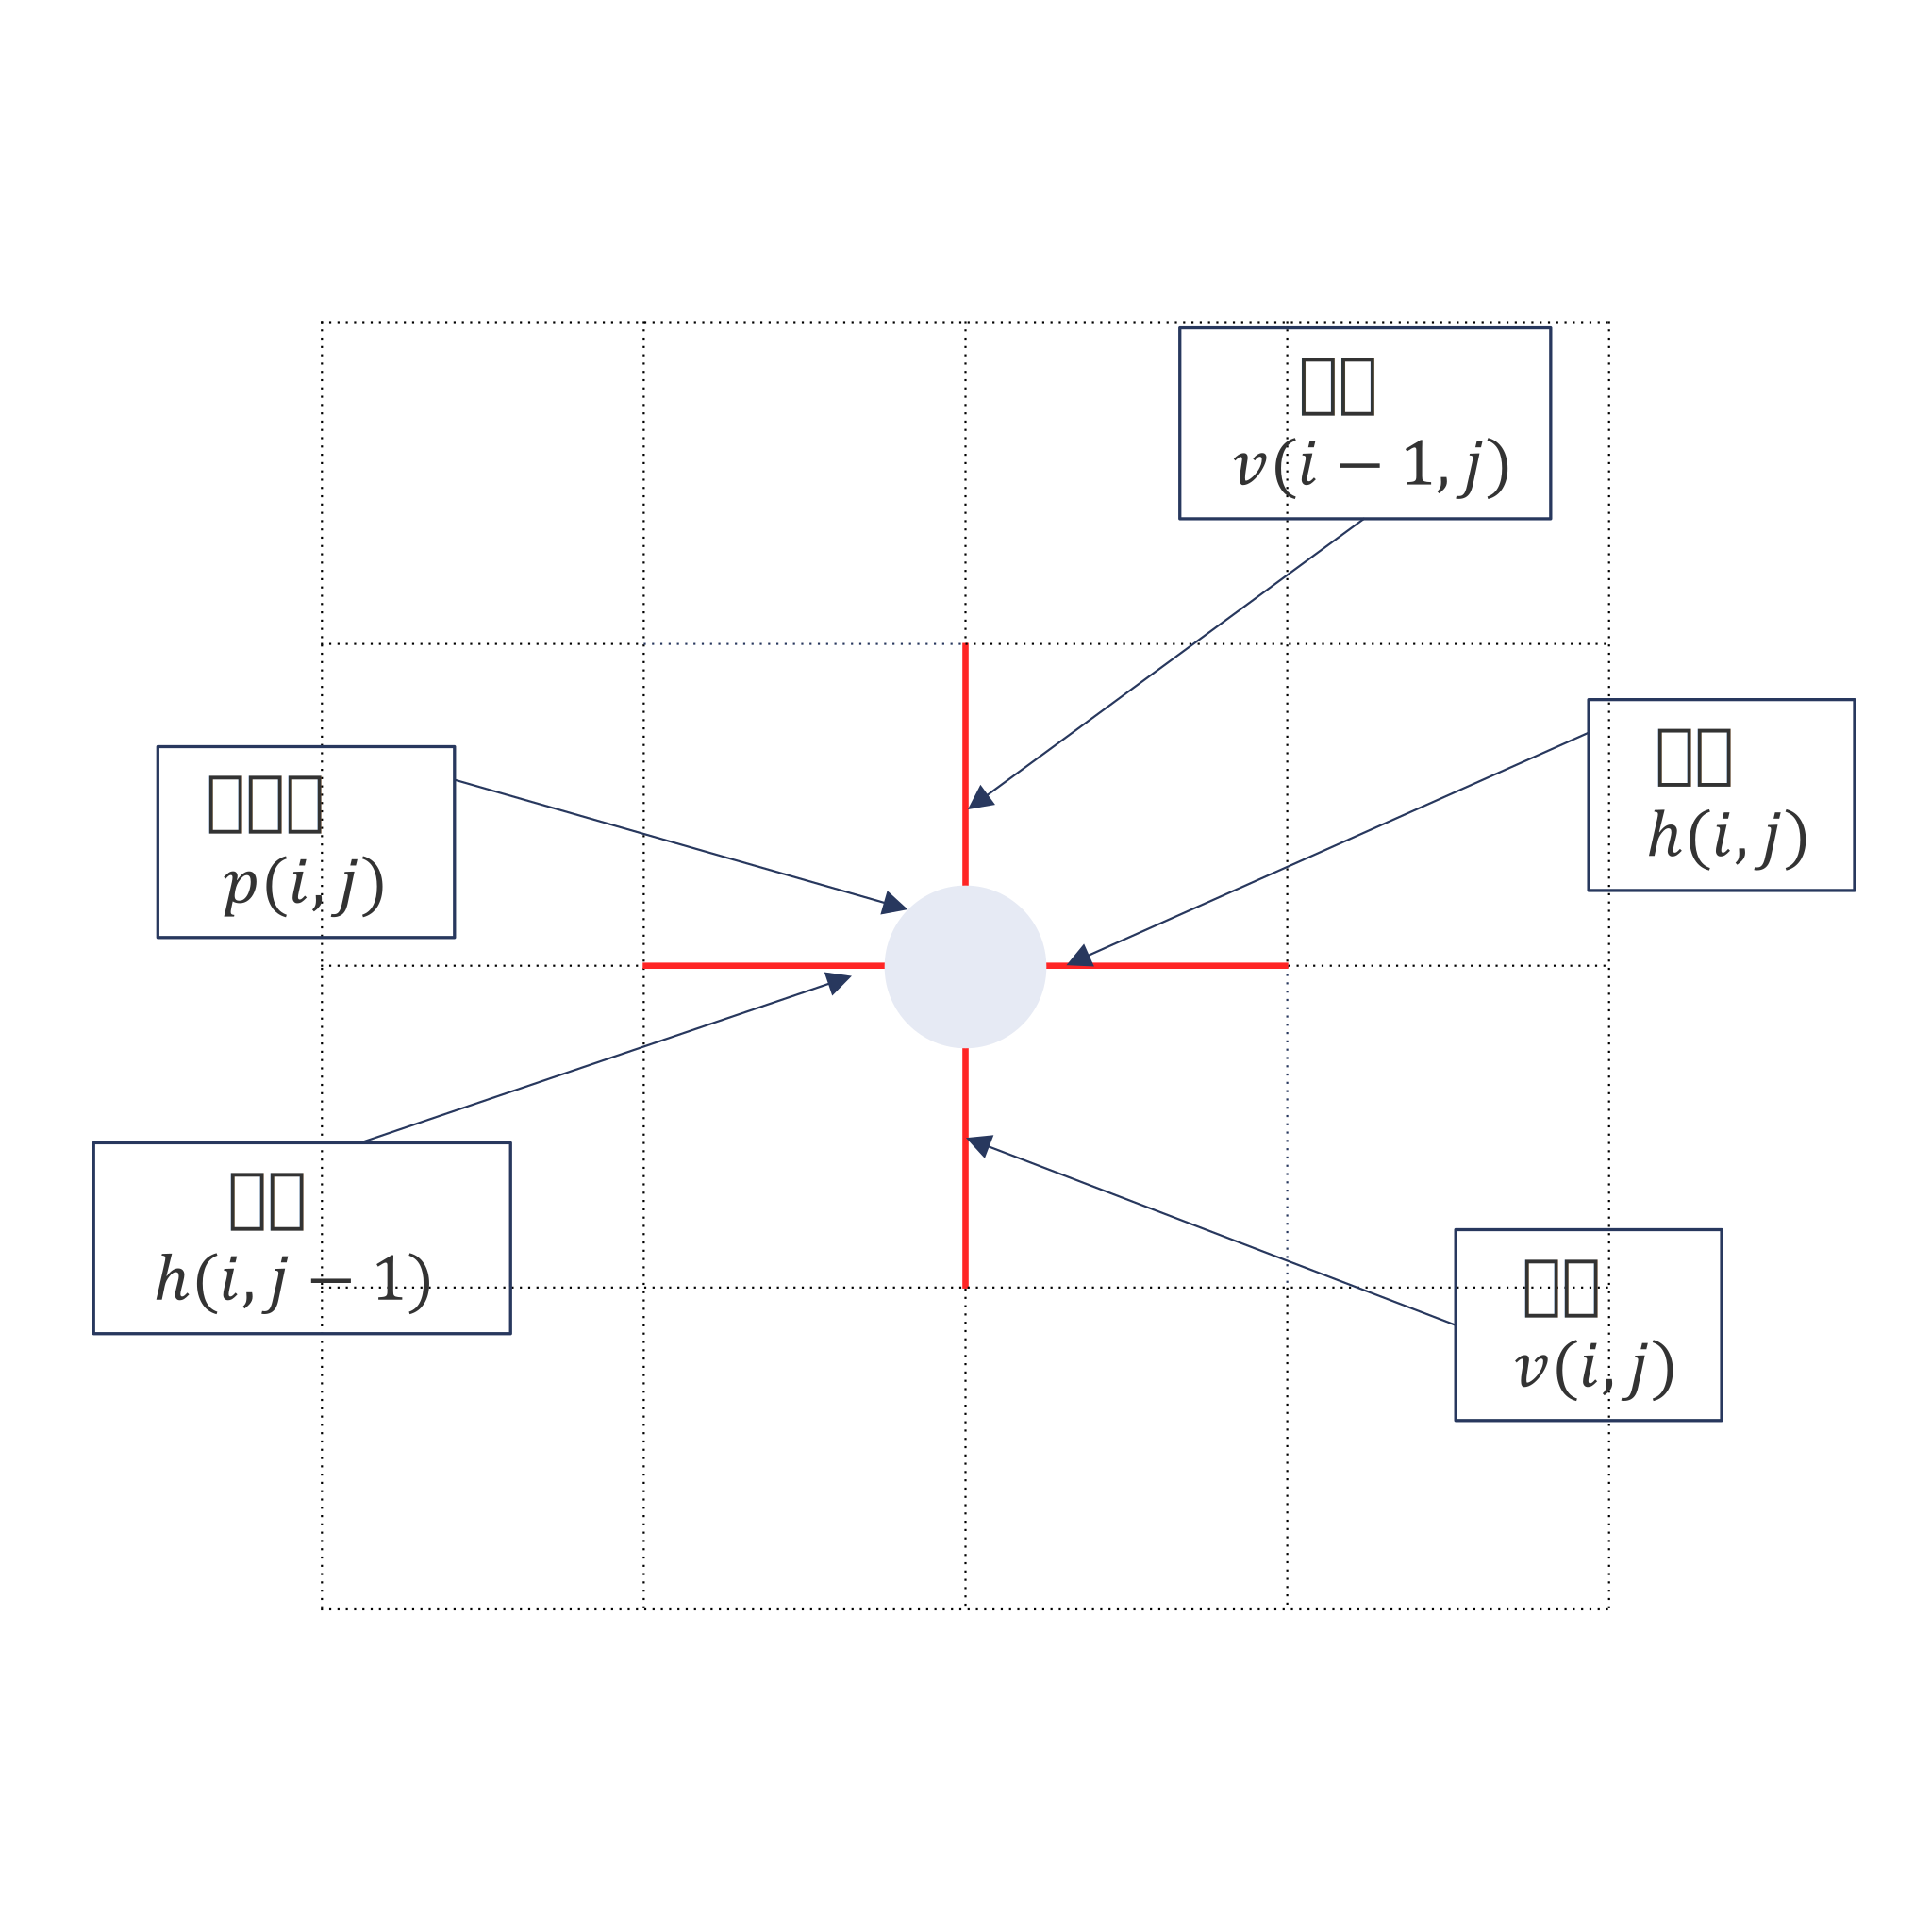
\includegraphics[width=5cm]{fig/cross.png}
  \caption{cross(イメージのためにつけておきます.)}
\end{figure}

\begin{figure}[htbp]\label{fig:cycle}
  \centering
  \includegraphics[width=5cm]{fig/cycle.png}
  \caption{cycle(イメージのためにつけておきます.)}
\end{figure}


\subsection{盤面上の変数の関係性の定義}\label{subsection:RelationDefinition}

次に,前節で定義した盤面上の変数同士の関係性について定義を行う.ただし,ここでは完成盤面を仮定する.

まず,連結と含有の定義を行う.連結とは直感的に辺と辺が繋がっていることを表す用語とし,含有とは盤面上の変数が集合として他の変数を含むことを表す用語として導入する.

\begin{definition}\textup{\textgt{連結}}

  \begin{equation}
    \begin{aligned}
                & e(i,j)とe(i',j')が連結である \\
      \coloneqq &
      \left\{
      \begin{aligned}
         & e_{i,j}=1, e_{i',j'}=1             & \\
         & e(i,,j)\cup e(i',j')\neq \emptyset &
      \end{aligned}
      \right.
    \end{aligned}
  \end{equation}
\end{definition}

\begin{definition}\textup{\textgt{含有}}

  \begin{equation}
    \begin{aligned}
                & e(i,j)がp(i',j')を含む \\
      \coloneqq &
      \left\{
      \begin{aligned}
         & e_{i,j}=1              & \\
         & e(i,j)\supset p(i',j') &
      \end{aligned}
      \right.
    \end{aligned}
  \end{equation}
  \vskip\baselineskip
  \begin{equation}
    \begin{aligned}
                & c(i,j)がe(i',j')を含む \\
      \coloneqq &
      \left\{
      \begin{aligned}
         & e_{i',j'}=1            & \\
         & c(i,j)\supset e(i',j') &
      \end{aligned}
      \right.
    \end{aligned}
  \end{equation}
  \vskip\baselineskip

  \begin{equation}
    \begin{aligned}
                & c(i,j)がp(i',j')を含む \\
      \coloneqq &
      \begin{aligned}
        c(i,j)\supset p(i',j') &
      \end{aligned}
    \end{aligned}
  \end{equation}
\end{definition}
\vskip\baselineskip

さらに,「辿ることが出来る」という用語の定義を行う.

\begin{definition}\textup{\textgt{辿ることが出来る}}
  \begin{equation}
    \begin{aligned}
                & e(i,j)からe(i',j')に辿ることが出来る \\ \\
      \coloneqq &
      \begin{aligned}[t]
         & e_(i,j)と連結なe(i_1,j_1),e(i_1,j_1)と連結なe(i_2,j_2),...,                   \\
         & e(i_t,j_t)と連結なe(i',j')のような集合\{e(i_1,j_1),e(i_2,j_2),...,e(i_t,j_t)\}が \\
         & ただ1つでも存在すること
      \end{aligned}
      \\
                & ただし,自分自身は常に辿ることが出来るものとする.
    \end{aligned}
  \end{equation}
\end{definition}

\vskip\baselineskip
以上の定義を用いることによって,新たに「線」という概念を導入することができる.

\begin{definition}\textup{\textgt{線}}
  \begin{equation}
    \begin{aligned}
                & 線L=\{e(i,j)\} \\
      \coloneqq &
      \begin{aligned}
        L\ni \forall e(i,j),\forall e(i',j')が,いつでも互いに辿ることができるような集合\{e(i,j)\}
      \end{aligned}
    \end{aligned}
  \end{equation}
\end{definition}

\vskip\baselineskip

この線という概念も含有という概念を定義することができて,

\begin{definition}\textup{\textgt{線の含有}}

  \begin{equation}
    \begin{aligned}
                & LがL'を含む \\
      \coloneqq &
      \begin{aligned}
         & L\supset L' &
      \end{aligned}
    \end{aligned}
  \end{equation}

  \begin{equation}
    \begin{aligned}
                & Lがe(i,j)を含む \\
      \coloneqq &
      \begin{aligned}
         & L\supset  e(i,j) &
      \end{aligned}
    \end{aligned}
  \end{equation}

  \begin{equation}
    \begin{aligned}
                & Lがp(i,j)を含む \\
      \coloneqq &
      \begin{aligned}
         & L\ni \exists e(i,j)がp(i,j)を含む &
      \end{aligned}
    \end{aligned}
  \end{equation}


\end{definition}


\subsection{グラフの定義}\label{subsection:GraphDefinition}
前節\ref{subsection:RelationDefinition}で定義した概念を用いることによって,盤面$\Bigl\{\{p_{i,j}\},\{c_{i,j}\},\{e_{i,j}\}\Bigr\}$を与えたとき,盤面上にグラフという概念を導入することができる.

\begin{definition}\textup{\textgt{グラフ}}
  \begin{equation}
    \begin{aligned}
                & グラフG_x                                              \\
      \coloneqq &
      \begin{aligned}
        \{P_x,L_x\}=\biggl\{  \Bigl\{p(i,j)\Bigr\}_x,\Bigl\{e(i,j)\Bigr\}_x\biggr\}
      \end{aligned}
      \\\\
                & L_xはあるe(i,j)が存在したとき盤面上に存在するe(i,j)を含む線の中で最大の線であり,    \\
                & P_xはL_xが含む全てのp(i,j)の和集合とする.                         \\
                & ただし,どの線にも含まれないp(i,j)もグラフと呼び,その時に限りG_x=\{p(i,j)\}とし, \\
                & 孤立点と呼ぶこととする(\{p(i,j)\}は
      集合として,1つの要素p(i,j)しか持たない集合).
    \end{aligned}
  \end{equation}
\end{definition}

\vskip\baselineskip
このようなグラフという概念が盤面に存在すると考えられ,盤面上のグラフ全てを要素に持つ集合
\begin{equation}
  A=\{G_1,G_2,...,G_m\}=\{G_x\}\quad (mは盤面に存在するグラフの数)
\end{equation}
がいつでも一意に定まる.(証明\ref{subsection:GraphIsUniqueProof})
また,(定義\ref{definition:Function})で取り上げた関数のうち,グラフが定義に$p(i,j)$を含むことにより$\bm{cross}$に関しては「グラフ内の全ての$p(i,j)$において,$\bm{cross}(p(i,j))=2$」などという条件を構成できる.


\begin{example}\textup{スリザーリンクの$\mathbf{conditions}$}\label{example:SlitherLinkConditions}
  \begin{equation}
    \mathbf{conditions}\colon
    \left\{
    \begin{aligned}
       & B\in \forall p(i,j)   ,  c_{i,j} & , & \bm{cross}(p(i,j))=c_{i,j} & \\
       & G_1\in \forall p(i,j)            & , & \bm{cross}(p(i,j))=2       & \\
       & G_xは孤立点(x\geq 2)                 &
    \end{aligned}
    \right.
  \end{equation}
\end{example}
